\chapter{Máximos e mínimos}

\resumo{%
\begin{itemize}[label=\color{chapterscolor}\textbullet]
\item Entender o conceito de máximos e mínimos globais e locais.
\item Condição necessária para mínimos locais.
\item Entender o conceito de pontos críticos, e que nem todo ponto crítico é de máximo ou de mínimo.    
\end{itemize}
}


Consideremos a função 
\begin{equation}\label{eq:minimo_global}
f(x,y)=x^2+y^2.
\end{equation}
Claramente essa função nunca atinge valores negativos, isto é, $f(x,y)\geq 0$ para todo $(x,y)\in \R^2$. Além disso, $f$ atinge o valor 0 na origem. Resumindo:
$$f(x,y)=x^2+y^2\geq 0 = f(0,0).$$
Ou seja, a imagem dessa função é um intervalo limitado inferiormente por 0 (e 0 pertence de fato ao intervalo). 

Esse exemplo ilustra o conceito de mínimo global. 
\begin{definition}{Mínimo global ou absoluto}{def_min_global}
Um ponto \((x_1^0, x_2^0, \ldots, x_n^0)\) é considerado um \textit{mínimo global}\index{minimo@mínimo!global} de uma função \(f:D\subset\R^n\to\R\) se, para qualquer ponto \((x_1, x_2, \ldots, x_n)\in D\) tem-se \(f(x_1^0, x_2^0, \ldots, x_n^0) \leq f(x_1, x_2, \ldots, x_n)\). 
\end{definition}
Em outras palavras, a função atinge seu valor mínimo no ponto \((x_1^0, x_2^0, \ldots, x_n^0)\) do seu domínio. 

Considere agora a função 
\begin{equation}\label{eq:maximo_global}
{f}(x,y)=e^{-x^2-y^2}.
\end{equation}
Nesse caso, podemos determinar facilmente que $f(x,y)\leq 1 $, pois a imagem da função exponencial está limitada entre 0 e 1 se o argumento da exponencial é negativo, como é o caso. Observe também que a exponencial com argumento negativo atinge o valor quando tal argumento é zero, que acontece no caso dessa função apenas quando $(x,y)=(0,0)$.
Em resumo:
$${f}(x,y)\leq 1 = f(0,0). $$
Isto é, a imagem dessa função está limitada superiormente por 1. 

Tal exemplo ilustra a definição de máximo global.
\begin{definition}{Máximo global ou absoluto}{}
Um ponto \((x_1^0, x_2^0, \ldots, x_n^0)\) é considerado um \textit{máximo global}\index{maximo@máximo!global} de uma função \(f:D\subset \R^n\to \R\) se, para qualquer ponto \((x_1, x_2, \ldots, x_n)\in D\) tem-se \(f(x_1^0, x_2^0, \ldots, x_n^0) \geq f(x_1, x_2, \ldots, x_n)\).
\end{definition}

Em outras palavras, a função atinge seu valor máximo no ponto \((x_1^0, x_2^0, \ldots, x_n^0)\) do seu domínio. 


No caso da função definida em \eqref{eq:minimo_global}, sabemos que seu gráfico é o paraboloide de equação $z=x^2+y^2$. Que a origem seja um mínimo global dessa função significa geometricamente que a altura mínima atingida pelos pontos sobre o paraboloide é 0. 
\begin{figure}[!htb]
    \centering
\tdplotsetmaincoords{70}{110} % Adjust the view angles (azimuth, elevation)
    \begin{tikzpicture}[tdplot_main_coords,scale=3.0]
		\pgfmathsetmacro{\tini}{0.5*pi}
		\pgfmathsetmacro{\tfin}{1.85*pi}
		\pgfmathsetmacro{\tend}{2.5*pi}
		%%% Coordinate axis
		\draw[-latex] (0,0,0) -- (1.5,0,0) node [below left] {$x$};
		\draw[dashed] (0,0,0) -- (-1.25,0,0);
		\draw[-latex] (0,0,0) -- (0,1.5,0) node [right] {$y$};
		\draw[dashed] (0,0,0) -- (0,-1.25,0);

  
		\foreach \altura in {0.0125,0.025,...,1.0}{
			\pgfmathparse{sqrt(\altura)}
			\pgfmathsetmacro{\radio}{\pgfmathresult}
			\draw[blue!50,opacity=0.5] plot[domain=\tini:\tfin,smooth,variable=\t] ({\radio*cos(\t r)},{\radio*sin(\t r)},{\altura}); 
		}

  % segunda parte do eixo z
		\draw[-latex] (0,0,0) -- (0,0,1.75) node [above] {$z$};	
  
		\foreach \altura in {0.0125,0.025,...,1.0}{
			\pgfmathparse{sqrt(\altura)}
			\pgfmathsetmacro{\radio}{\pgfmathresult}
			\draw[blue!50,opacity=0.5] plot[domain=\tfin:\tend,smooth,variable=\t] ({\radio*cos(\t r)},{\radio*sin(\t r)},{\altura}); 
		}

	\end{tikzpicture}
        \caption{Paraboloide de equação $z=x^2+y^2$.}
    \label{fig:enter-label}
\end{figure}





Por outro lado, o gráfico da função definida em \eqref{eq:maximo_global} é a superfície conhecida como \textit{Gaussiana}, e mostramos que as alturas dos pontos que estão sobre a Gaussiana não excede o valor 1. 
\begin{figure}[!htb]
\centering
\tdplotsetmaincoords{70}{110} % Adjust the view angles (azimuth, elevation)
    \begin{tikzpicture}[tdplot_main_coords,scale=2.5]
		\pgfmathsetmacro{\tini}{0.5*pi}
		\pgfmathsetmacro{\tfin}{1.85*pi}
		\pgfmathsetmacro{\tend}{2.5*pi}
		%%% Coordinate axis
		\draw[-latex] (0,0,0) -- (1.5,0,0) node [below left] {$x$};
		\draw[dashed] (0,0,0) -- (-1.25,0,0);
		\draw[-latex] (0,0,0) -- (0,1.5,0) node [right] {$y$};
		\draw[dashed] (0,0,0) -- (0,-1.25,0);

  
		\foreach \altura in {0.0125,0.025,...,1.0}{
			\pgfmathparse{sqrt(-ln(\altura))}
			\pgfmathsetmacro{\radio}{\pgfmathresult}
			\draw[blue!50,opacity=0.5] plot[domain=\tini:\tfin,smooth,variable=\t] ({\radio*cos(\t r)},{\radio*sin(\t r)},{\altura}); 
		}
  

%segunda parte do eixo z	
 \draw[-latex] (0,0,0) -- (0,0,1.25) node [above] {$z$};	

  
  \foreach \altura in {0.0125,0.025,...,1.0}{
			\pgfmathparse{sqrt(-ln(\altura))}
			\pgfmathsetmacro{\radio}{\pgfmathresult}
			\draw[blue!50,opacity=0.5] plot[domain=\tfin:\tend,smooth,variable=\t] ({\radio*cos(\t r)},{\radio*sin(\t r)},{\altura}); 
		}

  \draw(0,0,1) node[above left]{$1$};
	\end{tikzpicture}
 \caption{A gaussiana de equação é $z=e^{-x^2-y^2}$.}
\end{figure}

Gostaríamos de ressaltar que a palavra \textit{global} nas definições  \ref{def_min_global} e \ref{def_max_global} não significa unicidade, senão que esses são os valores extremos da função globalmente sobre todo o seu domínio. Vejamos um exemplo que ilustra essa observação. 
\begin{example}{}{}
Consideremos agora a função $f(x,y)=\sen x\sen y$. 
Da expressão da função deduzimos que $f$ é limitada inferiormente por -1 e superiormente por $1$. Além disso, $f$ atinge o valor $-1$ em infinitos pontos da forma $\left(\frac{3\pi}{2}+2k\pi,\frac{3\pi}{2}+2k\pi\right)$ com $k\in\R$, todos, portanto, são mínimos globais. Analogamente, os pontos da forma $\left(\frac{\pi}{2}+2k\pi,\frac{\pi}{2}+2k\pi\right)$ com $k\in\R$, são máximos globais da função. Veja o gráfico de $f$ a seguir. 
\begin{figure}[H]
    \centering
    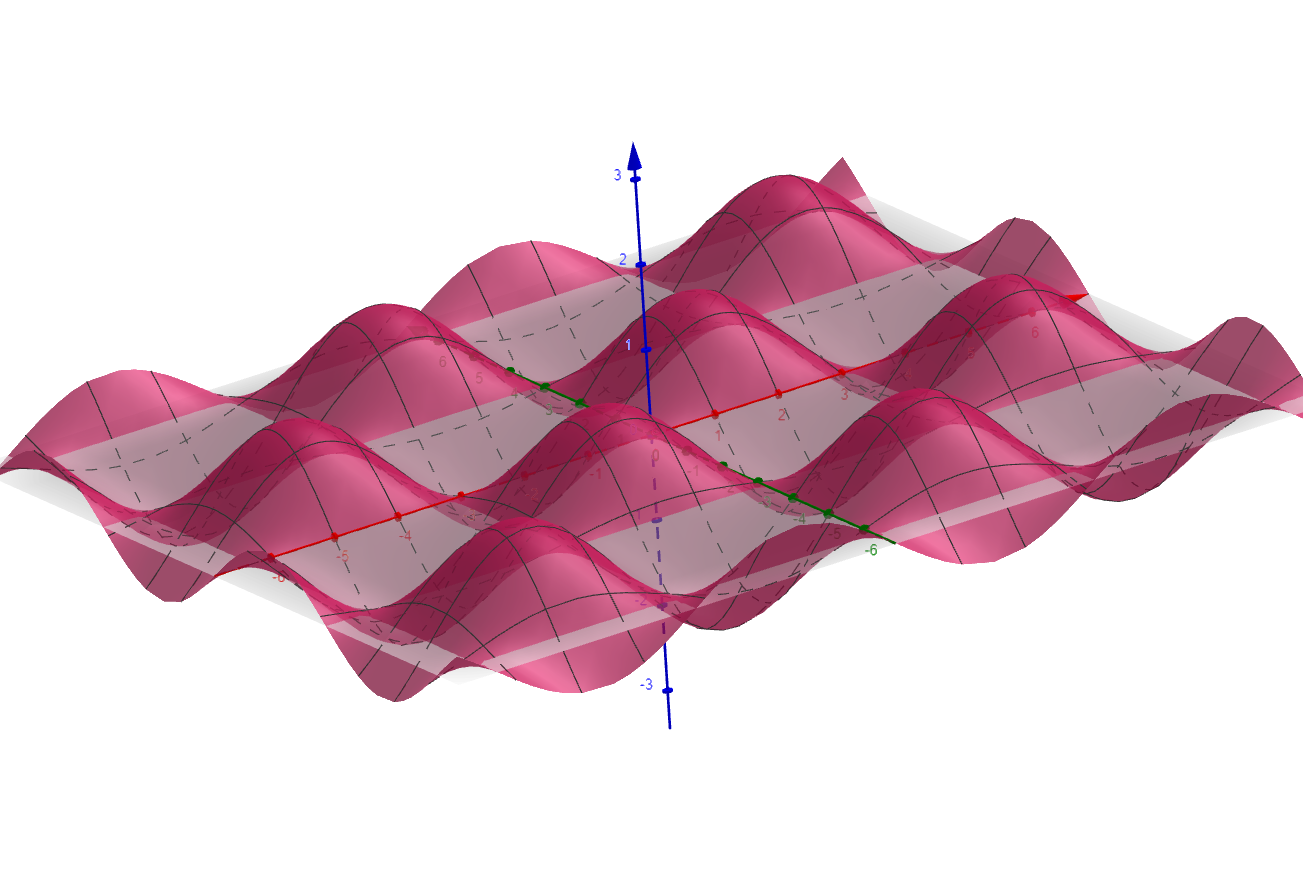
\includegraphics[scale=0.2]{Figuras/Semana11/seno}
    \caption{}
    \label{fig:enter-label}
\end{figure}
\end{example}

Por outro lado, como já dizemos, em muitos problemas, os domínios matemáticos das funções não coincidem com o conjunto no qual nos interessa estudar uma determinada função. Pode ocorrer que um máximo global de uma função esteja localizado fora do nosso domínio de interesse, ou nem exista. No entanto, mesmo nessas situações, é possível identificar pontos em que, dentro de vizinhanças limitadas desses pontos, os valores da função se mantêm sempre acima ou abaixo do valor da função no próprio ponto. Vejamos um exemplo.
\begin{example}{}{}
Seja $f(x,y)=(x^2+y^2)\ln(9-x^2-y^2)$. Pelas propriedades do logaritmo sabemos que $f$ é não negativa sobre o círculo de raio 3. Além disso, dentro desse círculo a função atinge o valor $0$ apenas em $(0,0)$, sendo um mínimo global se restringimos a análise da função apenas a esse círculo. Por outro lado, a função vai para menos infinito quando $(x,y)\rightarrow (\pm \infty,\pm \infty)$ e, portanto, a origem não é um mínimo global da função. 
\begin{figure}[H]
    \centering
    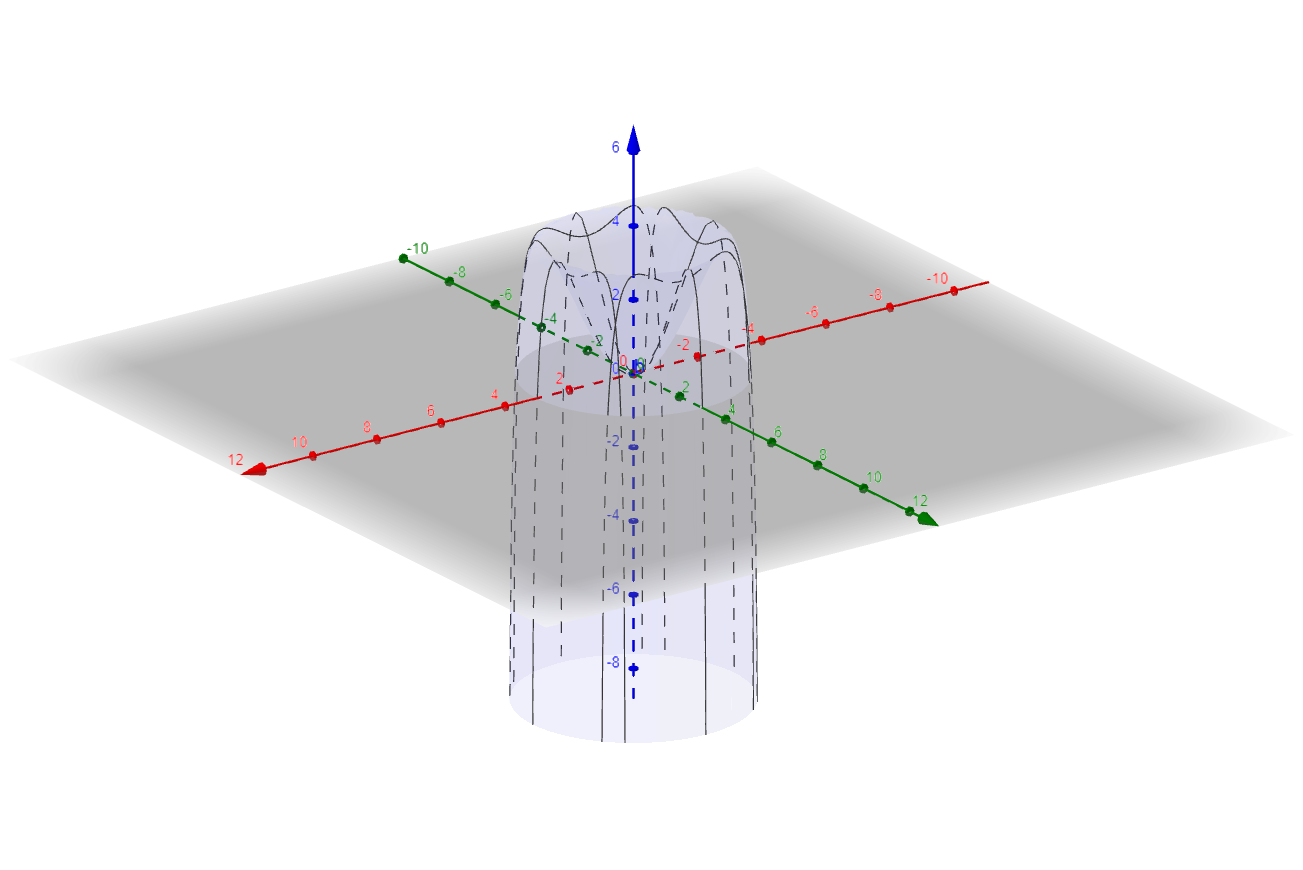
\includegraphics[width=\linewidth]{Figuras/Semana11/log_.png}
    \caption{}
    \label{fig:log}
\end{figure}
\end{example}

\pagebreak 
Esse tipo de pontos são de grande importância, pois,  embora não sejam extremos globais, podem ser suficientes para resolver determinado problema que esteja sendo  investigando. Se faz necessária, portanto, as seguintes definições. 
\begin{definition}{Mínimo local}{}
Um ponto \((x_1^0, x_2^0, \ldots, x_n^0)\) é considerado um \textit{mínimo local}\index{minimo@mínimo!local} de uma função \(f:D\subset\R^n\to\R\) se existe uma vizinhança em torno de \((x_1^0, x_2^0, \ldots, x_n^0)\) na qual \(f(x_1, x_2, \ldots, x_n)\leq f(x_1, x_2, \ldots, x_n)\) para todo $(x_1, x_2, \ldots, x_n)$ dentro dessa vizinhança, exceto possivelmente em \((x_1, x_2, \ldots, x_n)\) próprio.     
\end{definition}


Analogamente, temos o conceito de máximo local. 
\begin{definition}{Máximo local}{}
Um ponto \((x_1^0, x_2^0, \ldots, x_n^0)\) é considerado um \textit{máximo local}\index{maximo@máximo!local} de uma função \(f:D\subset\R^n\to\R\) se existe uma vizinhança em torno de \((x_1^0, x_2^0, \ldots, x_n^0)\) na qual \(f(x_1, x_2, \ldots, x_n)\geq f(x_1, x_2, \ldots, x_n)\) para todo $(x_1, x_2, \ldots, x_n)$ dentro dessa vizinhança, exceto possivelmente em \((x_1, x_2, \ldots, x_n)\) próprio.     
\end{definition}

Observe que os extremos globais em particular são extremos locais. 

\section{}
Até agora estudamos funções cujos valores extremos são facilmente determinados a partir da própria expressão da função. Em problemas da vida real, onde as funções modelam fenômenos complexos, é muito mais difícil determinar esses valores. Então precisamos buscar alternativas para determinar os pontos onde a função atinge seus extremos. O seguinte resultado é uma condição necessária satisfeita por extremos locais, que nos dá um primero passo na búsqueda por esses pontos. 
\begin{theorem}{}{}
    Se \((x_1^0, x_2^0, \ldots, x_n^0)\) é um {mínimo ou um máximo  local}\index{minimo@mínimo!local} de uma função diferenciável \(f:D\subset\R^n\to\R\), então $\nabla f(x_1^0, x_2^0, \ldots, x_n^0)=0$. 
\end{theorem}
\begin{proof}
Suponhamos que $\Point{x}_0=(x_1^0, x_2^0, \ldots, x_n^0)$ seja um mínimo local de $f$. Para cada $i=1,...,n$, consideremos a função de uma variável $$f_i(t)=f(x_1^0,\dots,x_{i-1}^0,x_i^0+t,x_{i+1}^0,\dots,x_n^0),$$ onde $t$ é suficientemente pequeno para que $(x_1^0,\dots,x_{i-1}^0,x_i^0+t,x_{i+1}^0,\dots,x_n^0)$ esteja contido em $D$. Obviamente $t=0$ é um mínimo dessa função, e de Cálculo I sabemos que $f_i'(0)=0$. Usando a regra da cadeia temos que 
$$f_i'(0) = \sum_{j=1}^n\dfrac{\partial f}{\partial x_j}(\Point{x}_0) \cdot x_j'(t) = \dfrac{\partial f}{\partial x_i}(\Point{x}_0). $$
Logo, todas as derivadas parciais são nula como desejado. 
\end{proof}



\todo[inline]{Observar aquí que o teorema implica que o plano tangente ao gráfico de uma função diferenciável nos seus máximos e mínimos locais é um plano horizontal porque o vetor normal é $N=(0,0,\dots,1)$.}

Observe que existem funções que podem não ser diferenciáveis nos seus pontos de máximo ou mínimo locais (ou globais). Por exemplo, a função de Cobb-Douglass, $u(x,y)=x^{\frac{1}{2}}y^{\frac{1}{2}}$, tem um mínimo global na origem e não é diferenciável na origem. A função $f(x,y)=\sqrt{x^2+y^2}$ também não é diferenciável na origem, que é seu mínimo global. Ou seja, o teorema pode ser aplicado às funções que sejam diferenciáveis, como indica a hipótese. Em outros casos são necessárias outras análises. 

\begin{example}{}{}
No caso da função definida em \eqref{eq:minimo_global}  temos que $\nabla f (x,y)=(2x,2y)$ que se anula na origem. No caso da função definida em \eqref{eq:maximo_global} temos $\nabla f(x,y)=\left(-2xe^{-x^2-y^2},-2ye^{-x^2-y^2}\right)$, que também se anula na origem. 
\end{example}

\begin{definition}{Ponto crítico}{}
    Um ponto $\Point{x}_0$ do domínio de uma função $f:D\subset \R^n\to\R$ de classe $C^2$ que satisfaz $\nabla f (\Point{x}_0)=0 $ é chamado de \textit{ponto crítico}\index{ponto!crítico} de $f$. 
\end{definition}

Observe agora que o Teorema 1.5 não diz que todo ponto crítico seja um máximo e um mínimo local. Vejamos um contraexemplo. 
\begin{example}{Sela de cavalo}{}
Considere a função    
\begin{equation}\label{eq:sela}
f(x,y)=x^2-y^2.
\end{equation}
Temos que $\nabla f(x,y)=(2x,-2y)$ que se anula na origem, porém, a origem não é nem um máximo nem um mínimo dessa função como vamos mostrar a continuação. 

Analizemos a curva plana que é interseção do gráfico de $f$ com o plano $y=0$, em vermelho na Figura \ref{fig:sela1}. 
\begin{figure}[H]
    \centering
    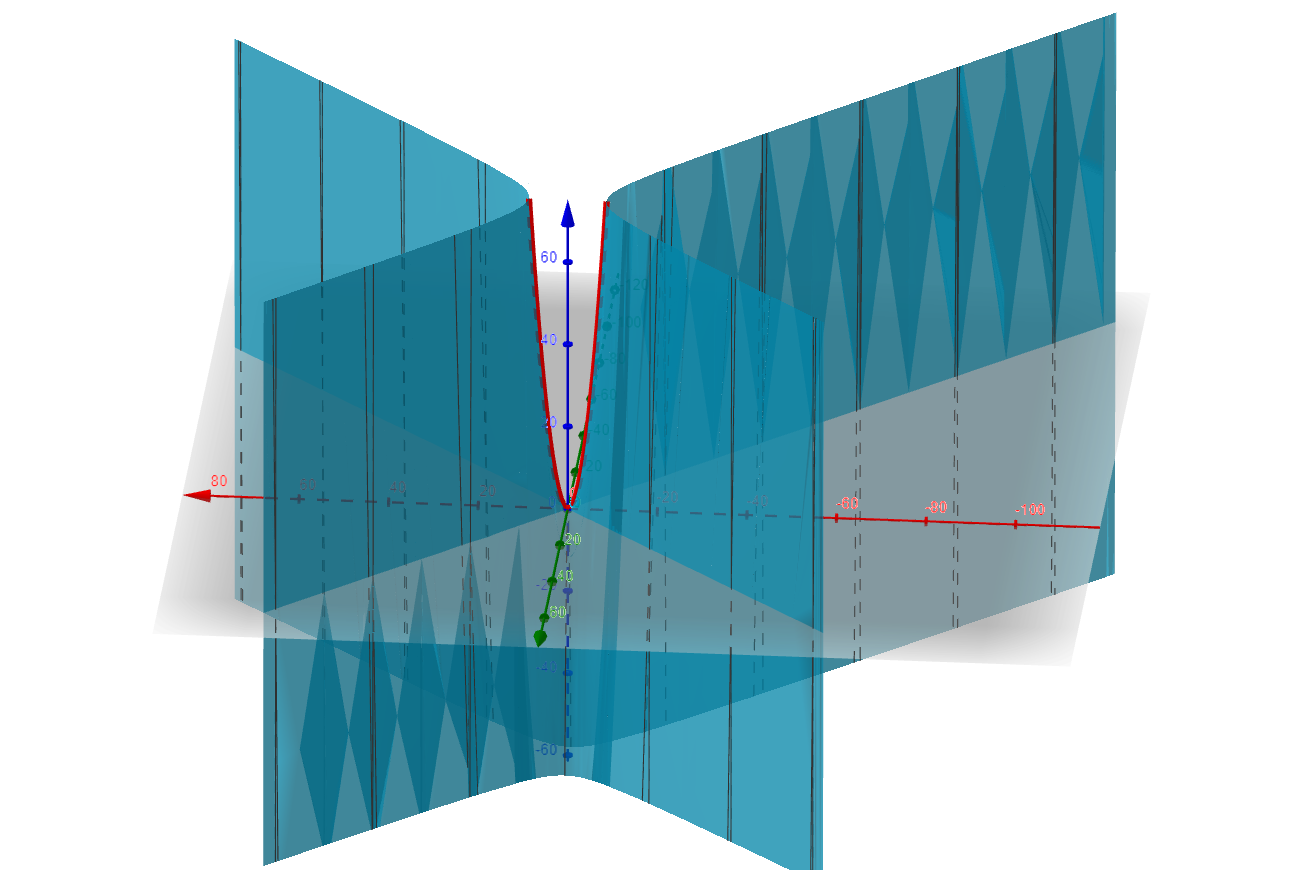
\includegraphics[scale=0.25]{Figuras/Semana11/sela1}
    \caption{}
    \label{fig:sela1}
\end{figure}
Visualmente observamos que essa curva tem uma altura mínima igual a zero, e de fato, no plano de equação $y=0$, tal curva é o gráfico da função de uma variável $h(x)=f(x,0)=x^2$, que obviamente tem um mínimo em $x=0$. Daí, sobre os pontos dessa curva temos
\begin{equation}
    f(x,0)=h(x)\geq h(0)=f(0,0).
    \label{eq:sela1}
\end{equation}
Por outro lado, na Figura \ref{fig:sela2} se mostra a curva que é o gráfico no plano de equação $x=0$ da função $\Tilde{h}(y)=f(0,y)=-y^2$, que tem um máximo em  $y=0$. 
\begin{figure}[H]
    \centering
    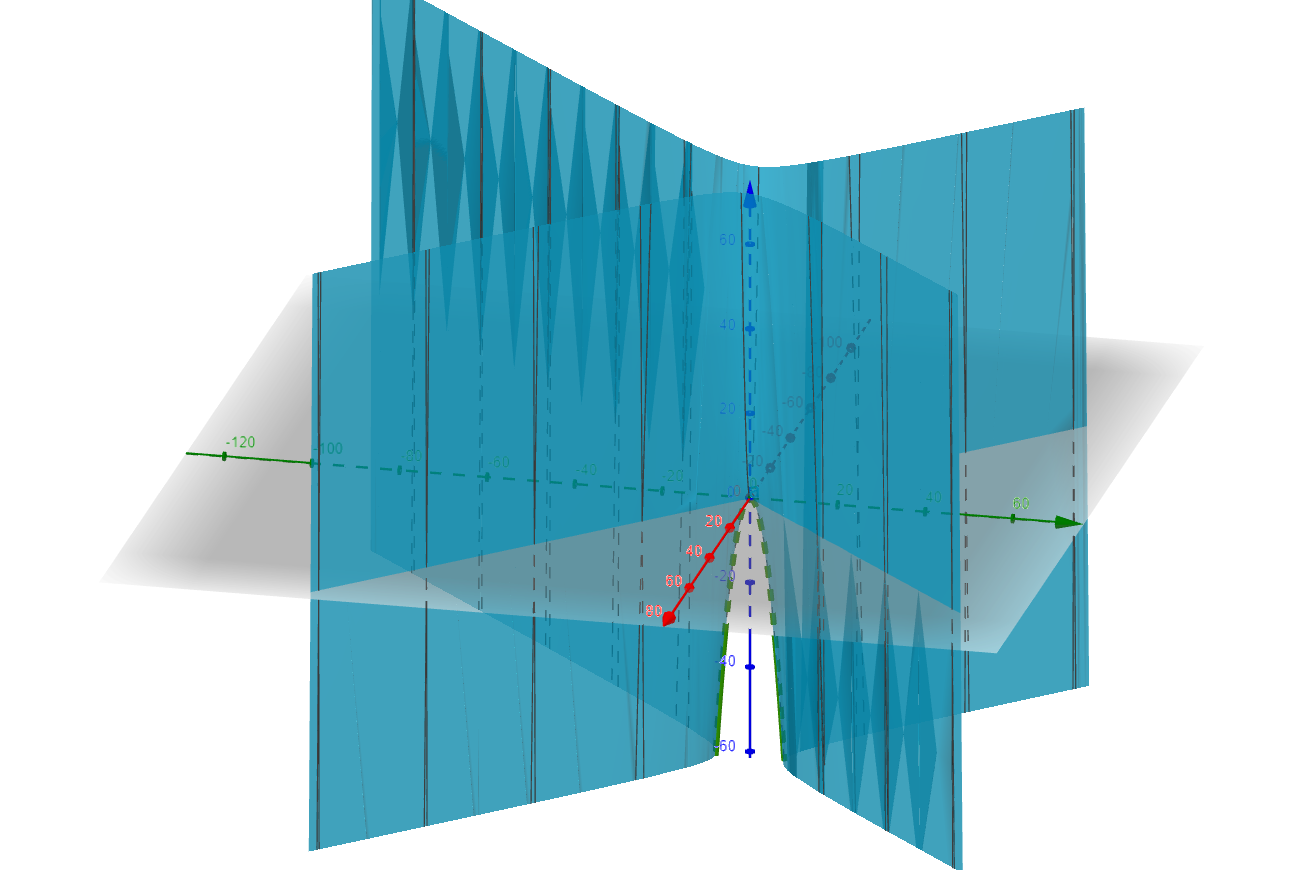
\includegraphics[scale=0.25]{Figuras/Semana11/sela2}
    \caption{}
    \label{fig:sela2}
\end{figure}
Desta forma, 
\begin{equation}
f(0,y)=\Tilde{h}(y)\leq \Tilde{h}(0)=f(0,0).
\label{eq:sela2}
\end{equation}

As equações \eqref{eq:sela1} e \eqref{eq:sela2} implicam que $(0,0)$ não é nem máximo nem mínimo dessa função, pois implicam que $f$ não satisfaz nem a definição de mínimo local nem a definição de máximo local. 
\end{example}

\begin{definition}{}{}
    Um ponto crítico de uma função que não é nem máximo e nem mínimo local é chamado de \textit{sela}\index{sela}.  
\end{definition}

\section{Classificação dos pontos críticos}
O Teorema 1.4 fornece o primeiro passo na busca por extremos locais de uma função diferenciável. No entanto, para determinar se um ponto crítico é um máximo ou mínimo, dependendo do contexto, precisamos de ferramentas adicionais.

Para isso, observemos que o Teorema de Taylor garante que se $\Point{x}_0=(x_1^0,x_2^0,\dots,x_n^0)$ é um ponto crítico de uma função duas vezes diferenciável $f:D\subset\R^n\to\R$, então para todo $\Point{x}=(x_1,x_2,\dots,x_n)$ suficientemente próximo de $\Point{x}_0$ temos que
\begin{align*}
\!\!f(\Point{x})-f(\Point{x}_0)&= \sum_{i=0}^n \underbrace{\dfrac{\partial f}{\partial x_i} (\Point{x}_0)}_{0} (x_i-x_i^0) + \frac{1}{2}\sum_{i,j=1}^n \dfrac{\partial ^2 f}{\partial x_i \partial x_j}(\Point{x}_0)(x_i-x_i^0)(x_j-x_j^0) + R(\Point{x})\\
&= \frac{1}{2} \sum_{i,j=1}^n \dfrac{\partial ^2 f}{\partial x_i \partial x_j}(\Point{x}_0)(x_i-x_i^0)(x_j-x_j^0) + R(\Point{x})
\end{align*}
sendo que
\begin{equation}\label{eq:resto}
    \lim_{\Point x \rightarrow \Point{x}_0} \dfrac{R(\Point{x})}{\|\Point{x}-\Point{x}_0\|^2}=0. 
\end{equation}

Se a forma quadrática 
$$Q(\Point{x})=\sum_{i,j=1}^n \dfrac{\partial ^2 f}{\partial x_i \partial x_j}(\Point{x}_0)x_i x_j=\Point{x}^T \Hess f(\Point{x}_0)\Point{x}$$
for estritamente definida positiva, isto é, se $Q(\Point{x})>0$ para todo $\Point{x}\neq 0$, então $\Point{x}_0$ é um mínimo local. De fato, como
$$\lim_{\Point x \rightarrow \Point{x}_0} \dfrac{Q(\Point x -  \Point{x}_0)}{\norm{\Point x -  \Point{x}_0}^2} > 0$$
e vale \eqref{eq:resto}, então podemos ``encolher'' a vizinhança em torno de $\Point{x}_0$ de forma tal que  
$$f(\Point{x})-f(\Point{x}_0)=Q(\Point{x}-\Point{x}_0)-R(\Point{x})>0.$$ 

Analogamente, se $Q$ for estritamente definida negativa temos que $\Point{x}_0$ é um máximo local. 

\begin{example}{}{}
Observe como no caso da função definida em \eqref{eq:minimo_global} temos que 
$$\Hess f(0,0)= \begin{pmatrix}
    2&0\\
    0&2
\end{pmatrix},$$
logo,
$$Q(x,y)=2x^2+2y^2,$$
que é estritamente positiva para todo $(x,y)\neq (0,0)$. De qualquer forma, já sabíamos que a origem é um mínimo global. 

Analogamente, para a função definida em \eqref{eq:maximo_global} temos que 
$$\dfrac{\partial^2 f}{\partial x^2}(x,y)=-2(1-2x^2)e^{-x^2-y^2},$$
$$\dfrac{\partial^2 f}{\partial x \partial y}(x,y)=\dfrac{\partial^2 f}{\partial y \partial x}(x,y)=4xye^{-x^2-y^2}$$
e
$$\dfrac{\partial^2 f}{\partial x^2}(x,y)=-2(1-2y^2)e^{-x^2-y^2}.$$
Assim, 
$$\Hess f(0,0)= 
\begin{pmatrix}
    -2&0\\
    0&-2
\end{pmatrix}$$
e, portanto, 
$$Q(x,y) = -2x^2-2 y^2$$
que é estritamente negativa fora da origem. 
\end{example}
Para aqueles que já possuem conhecimento sobre autovalores de matrizes, observem que em ambos os casos do exemplo anterior a matriz Hessiana é a matriz diagonal contendo um único autovalor de multiplicidade 2. Lembrem que para determinar se uma forma quadrática é estritamente definida positiva ou negativa é suficiente analisar o sinal dos autovalores da matriz que a representa. 

\pagebreak
Vejamos outro exemplo
\begin{example}{}{}
Consideremos a função
\begin{equation}\label{ilust_locais}
    f(x,y)=x^4+y^4 -4xy + 1
\end{equation} 

Temos
$$\nabla f (x,y) = (4x^3-4y,4y^3-4x).$$
Para determinar os pontos críticos devemos resolver os sistema de equações
$$\begin{cases}
    4x^3-4y=0,\\
    4y^3-4x=0,
\end{cases}$$
cujas soluções são $p_1=(1,1)$, $p_2=(-1,-1)$ e $p_3=(0,0)$. Para identificar quem é máximo e mínimo, devemos determinar a forma quadrática $Q$.
Temos 
$$\dfrac{\partial^2 f }{\partial x^2}(x,y)=12x^2,\quad 
\dfrac{\partial^2 f }{\partial x\partial y}(x,y)=\dfrac{\partial^2 f }{\partial y\partial x}(x,y)=-4 
\quad \mbox{e} \quad \dfrac{\partial^2 f }{\partial y^2}(x,y)=12 y^2.$$
Logo,
$$\Hess f(1,1)= \Hess f(-1,-1)=
\begin{pmatrix}
    12&-4\\
    -4&12
\end{pmatrix},$$
assim, em ambos casos temos que 
$$Q(x,y)=12x^2-8xy+12y^2.$$
Nesse caso não podemos determinar a simples vista se $Q$ tem um sinal bem definido. Façamos uma pequena análise:
Se $x=0$ temos que $Q>0$. Supondo agora que $x\neq 0 $ 
podemos considerar que $p(y)=3x^2-2xy+3y^2$ é um  polinômio em $y$ para cada $x$ fixado. Assim, o discriminante é 
$D= 4x^2 -4 \cdot 3 \cdot 3x^2 =-32 x^2<0,$ o que implica que tal polinômio não tem raízes reais. Isso significa que ele não muda de sinal e, portanto, $p(y)$ terá o mesmo sinal do caso em que $y=x$, ou seja, $p(x)=3x^2-2x\cdot x+3x^2=4x^2>0$. Como para cada $x$ fixado $Q(x,y)>0$ para todo $y\in\R$, concluímos que $Q(x,y)>0$ para todo $(x,y)\in\R^2$. Portanto $(1,1)$ e $(-1,-1)$ são mínimos locais. 

\medskip 

Por outro lado, 
$$\Hess f(0,0)= 
\begin{pmatrix}
    0&-4\\
    -4&0
\end{pmatrix}$$
Daí, 
$Q(x,y)=-8xy$ cujo sinal não é constante, depende do sinal de $x$ e de $y$. Observe na figura a seguir que a origem é uma sela. 


\begin{figure}[H]
    \centering
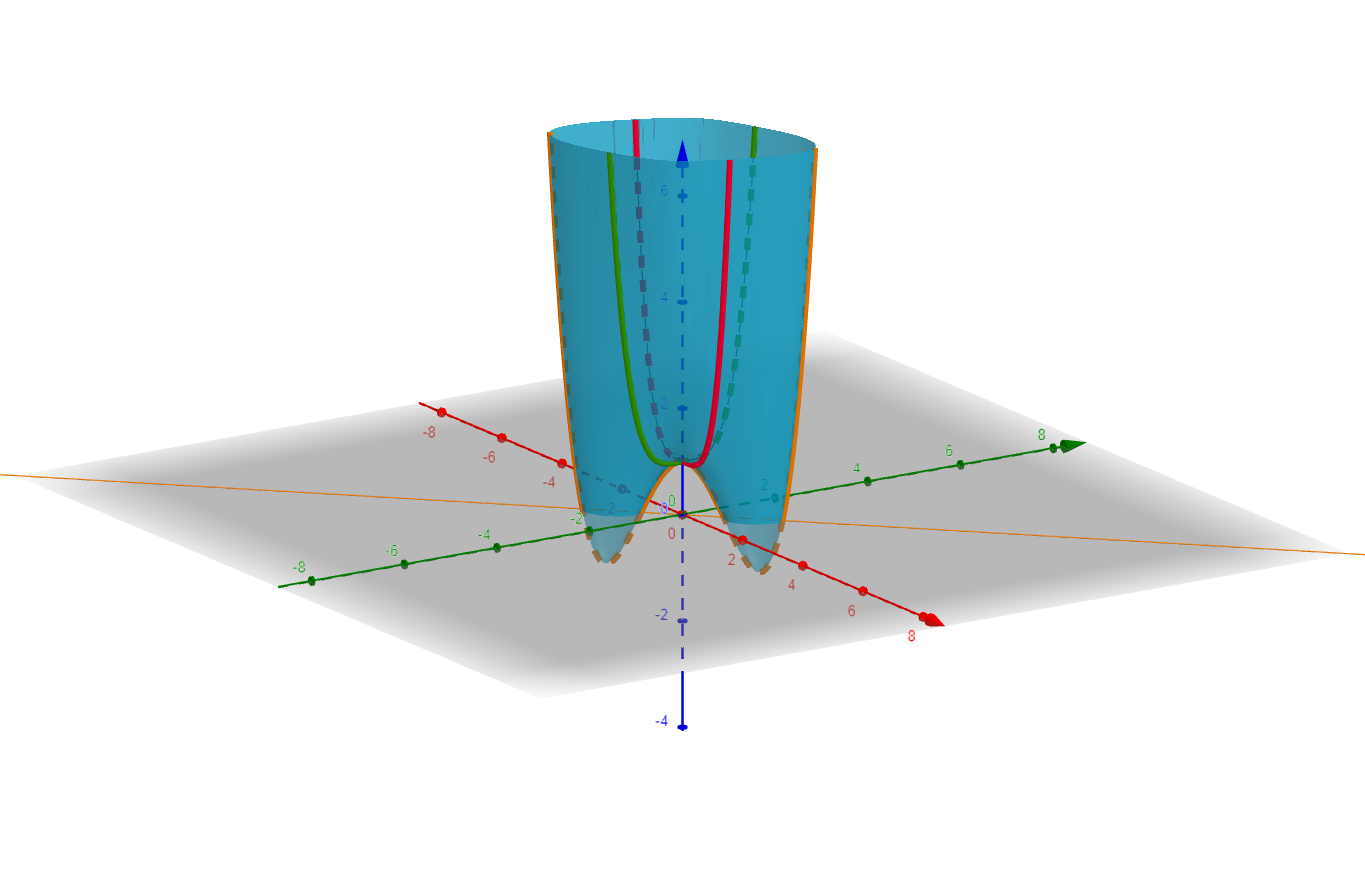
\includegraphics[scale=0.2]{Figuras/Semana11/fig1}
\end{figure}
\end{example}

No exemplo anterior, observamos que a determinação do sinal da forma quadrática $Q$ foi mais desafiadora em comparação ao Exemplo 1.5. Em situações gerais, a análise direta do sinal pode ser bastante complicada, senão impossível, dependendo da expressão da função em análise. Portanto, é de grande importância possuir métodos que permitam determinar se uma forma quadrática é positiva ou negativa sem depender de análises detalhadas.

Para chegar no caso geral, comecemos pelo caso em que $f$ é uma função de duas variáveis ($n=2$) e de classe $C^2$. Seja $(x_0,y_0)$ um ponto crítico, então
\begin{equation}\label{eq:q}
Q(x,y) =\frac{\partial^2f}{\partial x^2}(x_0,y_0)x^2 + 2 \frac{\partial^2f}{\partial x\partial y}(x_0,y_0)xy + \frac{\partial^2f}{\partial y^2}(x_0,y_0)y^2. 
\end{equation}
Façamos uma análise parecida com a que fizemos no Exemplo 1.6. Fixemos $x\neq 0$  e consideremos o seguinte polinômio em $y$:
$$p(y)=\frac{\partial^2f}{\partial x^2}(x_0,y_0)x^2 + 2 \frac{\partial^2f}{\partial x\partial y}(x_0,y_0)xy + \frac{\partial^2f}{\partial y^2}(x_0,y_0)y^2.$$
Temos
\begin{align*}
D & = \underbrace{4\left(\frac{\partial^2f}{\partial x\partial y}(x_0,y_0)\right)^2x^2}_{b^2}-4\cdot \underbrace{\frac{\partial^2f}{\partial y^2}(x_0,y_0)}_{a}\cdot \underbrace{\frac{\partial^2f}{\partial x^2}(x_0,y_0)x^2}_c.\\
&= -4x^2\left( \underbrace{\frac{\partial^2f}{\partial x^2}(x_0,y_0) \frac{\partial^2f}{\partial y^2}(x_0,y_0)-\left(\frac{\partial^2f}{\partial x\partial y}(x_0,y_0)\right)^2}_{\det \left(\Hess f(x_0,y_0)\right)}\right). 
\end{align*}
%Se $(x_0,y_0)$ for um máximo ou um mínimo, então $D$ tem que ser estritamente negativo, pois 
Observe que a condição ``$Q>0$ ou $Q<0$'' implica que $p(y)$ não tem raízes reais. Portanto, $\det \left(\Hess f(x_0,y_0)\right)$ tem que ser estritamente positivo. 

%Se $\det \left(\Hess f(x_0,y_0)\right)$ for não negativo, então $Q$ muda de sinal

Além disso, observe que se $\det \left(\Hess f(x_0,y_0)\right)>0$, então necessariamente $ \frac{\partial^2f}{\partial x^2}(x_0,y_0)$ e $ \frac{\partial^2f}{\partial x^2}(x_0,y_0)$ não se anulam e tem o mesmo sinal! Assim, $Q(x,y)$ tem o mesmo sinal que $Q(1,0)=\frac{\partial^2f}{\partial x^2}(x_0,y_0)$ (que é o mesmo sinal de $Q(0,1)=\frac{\partial^2f}{\partial y^2}(x_0,y_0)$). 

Chegamos, portanto, ao seguinte critério de classificação:
\begin{theorem}{Critério de classificação de pontos críticos para funções de duas variáveis}{}
Sejam $f:D\subset \R^2\to\R$ uma função de classe $C^2$ e $(x_0,y_0)\in D$ um ponto crítico de $f$. Então
\begin{itemize}
\item Se $\det (\Hess f(x_0,y_0))>0$ e $\frac{\partial^2f}{\partial x^2}(x_0,y_0)>0$, então $(x_0,y_0)$ é um mínimo local (pois $Q$ é estritamente definida positiva).
\item Se $\det (\Hess f(x_0,y_0))>0$ e $\frac{\partial^2f}{\partial x^2}(x_0,y_0)<0$, então $(x_0,y_0)$ é um máximo local (pois $Q$ é estritamente definida negativa).
\item Se $\det (\Hess f(x_0,y_0))<0$, então $(x_0,y_0)$ é uma sela. 
\end{itemize}
\end{theorem}

Observe que se $\det (\Hess f(x_0,y_0))=0$ não podemos dizer nada sobre a natureza do ponto crítico. %De fato, neste caso, $D=0$ e $p(y)$ teria uma única raiz para cada $x$ fixado, digamos $y_x$ (porque tal $y$ depende de $x$). Ou seja, para cada $x$ existe $y_x$ tal que  $Q(x,y_x)=0$. Mas isso não diz nada sobre o sinal de $Q$ poderia ser positivo sempre, neste caso necessariamente   

